\section{State of the art}
Arguably, Go is very well suited to be used as a state of the art reference in terms of web-centered concurrency implemented through user-space context-switching, especially when compared to a multi-procedural implementation in C. First of all, Go was created at Google in 2010 by some of the computer science pioneers that originally came up with Unix and C at Bell Labs, so it is no surprise that Go has been described as a "C-like language" or as "C for the 21st Century" \cite{GoPL2015}. Furthermore, it was created with "built-in concurrency" to tackle modern large distributed infrastructure problems and it is currently widely used at all network traffic levels as a server-side service provider \cite{Pike2012}\cite{Ajmani2016}\cite{2022DataRacesGolang}. Therefore, it is a great candidate as a point of reference of how modern server-side network concurrency can be handled \cite{GoArticleACM}, from which a totally different architecture based on blocking processes can be developed. 

If the main goal of this paper is to open a developer's eyes to the many different concurrency paradigms that can be used for server-side development, then the philosophy of Go (and for that matter, also of other popular frameworks like Node.js) is the antithesis of this work, because these frameworks provide an inflexible architecture that handles concurrency. In the case of Go, the syntax to handle the creation of concurrent workloads (so-called "\textit{goroutines}") and of communication channels between the goroutines is so simple that an unaware or beginner programmer might be completely oblivious of the scheduling work being performed under the hood by the Go runtime, or even of the fact that its code is running concurrently \cite{2022DataRacesGolang}. 

\subsection{Goroutines}
\begin{figure}[!t]
	\centering
	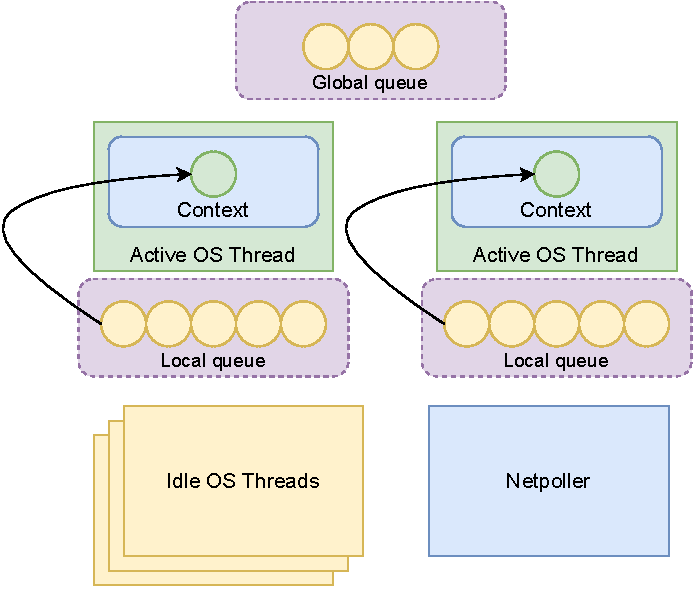
\includegraphics[width=2.5in]{img/go_runtime.pdf}
	%where an .eps filename suffix will be assumed under latex, 
	%and a .pdf suffix will be assumed for pdflatex; or what has been declared
	%via \DeclareGraphicsExtensions.
	\caption{High level depiction of the run-time environment in Go. \textit{Goroutines} are depicted as circles, OS threads as rectangles. Active goroutines running on a \textit{context} are green, idle goroutines waiting in a queue are yellow. The same color semantics apply to active and idle OS threads.}
	\label{fig_go_runtime}
\end{figure}
The idiomatic way of dealing with client connections in Go, either in an HTTP(s) server or through solely raw TCP communication, is by spawning a new goroutine that handles each client concurrently \cite{Morsing2013_2}\cite{GoNet}\cite{GoHTTP}. From a software engineering perspective this is a very practical approach, since it elevates the level of abstraction that the programmer has to deal with, so that it is unnecessary to directly intervene in memory synchronization and the management of a thread pool. This should have as a consequence gains in developer productivity, with the trade-off that there is less design freedom. The pledge of Go is that the run-time will single-handedly manage the scheduling of goroutines in the most effective way possible and that goroutines are so lightweight that the developer should not worry upfront about the amount of goroutines that would simultaneously be spawned \cite{2013ContextSwitching}\cite{Cox-Buday2017}.

Goroutines are very lightweight concurrent subroutines  supervised by the Go \textit{runtime} in user-space. Their memory footprint is very small \cite{2013ContextSwitching}, the assigned stack memory by default is only a few kilobytes at their creation \cite{Cox-Buday2017}. From the perspective of the kernel, goroutines are non-preemptive, i.e. they are not interrupted by the OS scheduler to run other goroutines. They have defined \textit{points of entry} where they can be suspended or activated by the run-time scheduler, which is entirely running in user-space. Since a context-switch between goroutines happens in user-space and the runtime decides which data should be persistent between context-switches, it is orders of magnitude faster than context-switching between OS threads \cite{Cox-Buday2017} or between OS processes \cite{Kerrisk2010}. A context-switch between OS threads or processes is a costly operation in terms of both the kernel-side data structures needed to maintain all threads and processes, the operations performed in kernel space to make the transition happen and, possibly, the shifting of memory blocks during the transition.

\subsection{Runtime scheduler}
Each Go executable is compiled with its own statically linked run-time environment in charge of scheduling the goroutines, garbage collection and other tasks. The system model that describes the runtime scheduler consists of three main elements: all statically and dynamically called goroutines, a context and the OS threads where the goroutines are run. Goroutines are placed by the run-time in either the local queue of a context or in the global queue pending to be run by a context in one of the OS threads, as illustrated in figure \ref{fig_go_runtime}. The contexts are in charge of managing the scheduling of the goroutine queues.

Parallelism in the system is achieved by having multiple contexts (in fig. \ref{fig_go_runtime} only two contexts are simultaneously running, depicted as blue rectangles), each using a different core of the processor through different OS threads, in order to run the  goroutines waiting in their queues. The runtime manages a set of working threads (illustrated as green rectangles) coupled with contexts and another set of idle threads (yellow rectangles).  If a goroutine performs a syscall that would block, e.g. listens for clients on a TCP socket, the overlying OS thread in which the context is executing the goroutine would also have to block. In this scenario, the blocking thread is decoupled from the context, so that the context can re-activate one of the idle threads and keep working with other non-blocking goroutines.

As long as the goroutines running in the contexts do not call a blocking system call, the different goroutines in the queues can be freely interchanged at the given \textit{points of entry} by the scheduler within the same set of OS threads. This, as previously stated, avoids a costly context-switch in kernel space. 

Nonetheless, blocking syscalls for networking are handled in a special way by the run-time. As previously stated, Go idiomatically creates a new goroutine for each client connected to a server. If the server were to have thousands of simultaneously connected clients and most of the clients were to call blocking system calls at the same time, it would then have to create a unique blocked OS thread for each client. This state would be very costly because every blocked client goroutine translates to one blocked OS thread, consequently defeating Go's goal of keeping context-switches primarily in userspace.

Therefore, Go handles network connections in a way that avoids using too many system resources. First, when a new connection is accepted by the server, its file descriptor is set in non-blocking mode, which means that if I/O is not possible in the network socket, the syscall returns an error, instead of automatically blocking. Hence, when a goroutine tries to perform I/O in a network socket and it returns an error, the goroutine notifies a special perpetually running thread called the "\textit{netpoller}", which polls the status of network sockets \cite{Morsing2013_2} (the netpoller thread is depicted as a blue rectangle in fig. \ref{fig_go_runtime}). The goroutine which could not perform its network operation is placed back on a queue (making its OS thread once again free to run another goroutine). The netpoller notifies a context when it is again possible to perform I/O in the file descriptor, so that the goroutine can be scheduled back in the future. Thereupon, the runtime environment avoids overloading the kernel with unnecessarily too many blocked threads for the client connections.